\documentclass[a4paper,12pt]{article}

%%%%%%%%%%%%%%%%%%%%%
% Small research about Asymmetry of Delta_CP

\usepackage[english]{babel}

 \usepackage[T1]{fontenc}
 \usepackage[colorlinks=false, urlcolor=black, breaklinks, pagebackref, citebordercolor={0 0 0}, filebordercolor={0 0 0}, linkbordercolor={0 0 0}, pagebordercolor={0 0 0}, runbordercolor={0 0 0}, urlbordercolor={0 0 0}, pdfborder={0 0 0}]{hyperref} 
%%%%%%%%%%%%%%%%%%%%% 
\usepackage{float}
\usepackage{amsmath}
\usepackage{amsfonts}
\usepackage{amssymb}
\usepackage{array}
%%%%%%%%%%%%%%%%%%%%%%%%%%
\usepackage{hyperref}
\makeatletter
\def\UrlAlphabet{%
      \do\a\do\b\do\c\do\d\do\e\do\f\do\g\do\h\do\i\do\j%
      \do\k\do\l\do\m\do\n\do\o\do\p\do\q\do\r\do\s\do\t%
      \do\u\do\v\do\w\do\x\do\y\do\z\do\A\do\B\do\C\do\D%
      \do\E\do\F\do\G\do\H\do\I\do\J\do\K\do\L\do\M\do\N%
      \do\O\do\P\do\Q\do\R\do\S\do\T\do\U\do\V\do\W\do\X%
      \do\Y\do\Z}
\def\UrlDigits{\do\1\do\2\do\3\do\4\do\5\do\6\do\7\do\8\do\9\do\0}
\g@addto@macro{\UrlBreaks}{\UrlOrds}
\g@addto@macro{\UrlBreaks}{\UrlAlphabet}
\g@addto@macro{\UrlBreaks}{\UrlDigits}
\makeatother
%%%%%%%%%%%%%%%%%%%%%%%%%%
\usepackage{hyperref}
\usepackage{geometry}
\usepackage{graphicx}
\usepackage{hyperref}
\usepackage{icomma}
\usepackage{latexsym}
\usepackage[numbers]{natbib}
\usepackage{textcomp}
\usepackage{tabularx}
\usepackage[all]{xy}
\usepackage{cancel}
\usepackage{color}
\usepackage{dsfont}
%\usepackage{subfig}
\usepackage{subfigure} 
\usepackage{caption}
\usepackage{dsfont}
\usepackage{extarrows}
\usepackage{shorttoc}
\usepackage{listings}
\usepackage[utf8]{inputenc}
\usepackage{lmodern}
\usepackage{xcolor}
\usepackage{moreverb}
\usepackage{float}
\lstset{language=scilab}

\lstset{
        basicstyle=\ttfamily,
        emphstyle=\color{blue},
        columns=flexible,
        breaklines=true,
        keywordstyle=\color{blue},
        commentstyle=\color{red},
}

   \newcommand{\bigO}[1]{\ensuremath{\mathop{}\mathopen{}O\mathopen{}\left(#1\right)}}
   \newcommand{\smallO}[1]{\ensuremath{\mathop{}\mathopen{}o\mathopen{}\left(#1\right)}}

\captionsetup{font=footnotesize}

\setcounter{tocdepth}{3}

\makeatletter
\def\clap#1{\hbox to 0pt{\hss #1\hss}}%
\def\ligne#1{%
\hbox to \hsize{%
\vbox{\centering #1}}}%
\def\haut#1#2#3{%
\hbox to \hsize{%
\rlap{\vtop{\raggedright #1}}%
\hss
\clap{\vtop{\centering #2}}%
\hss
\llap{\vtop{\raggedleft #3}}}}%
\def\bas#1#2#3{%
\hbox to \hsize{%
\rlap{\vbox{\raggedright #1}}%
\hss
\clap{\vbox{\centering #2}}%
\hss
\llap{\vbox{\raggedleft #3}}}}%
\def\maketitle{%
\thispagestyle{empty}\vbox to \vsize{%
\haut{}{\@blurb}{}
\vfill
\vspace{0.5cm}
\hrule height 2pt
\vspace{0.2cm}
\par
\begin{center}
\fontseries{bx}
\huge \@title
\end{center}
\vspace{0.2cm}
\par
\hrule height 2pt
\par
\vspace{2cm}
\begin{center}
\Large
\textit{}
\end{center}
\begin{center}
\Large 
\@author
\par
\end{center}
\vspace{1cm}
\begin{center}
\Large
\textit{}
\end{center}
\begin{center}
\Large 
Shuaixiang Zhang

Indiana University Bloomington
\par
\end{center}
\vfill
\vfill
\bas{}{\begin{flushright}
\large
\@location
\end{flushright}}{}
}%
\cleardoublepage
}
\def\date#1{\def\@date{#1}}
\def\author#1{\def\@author{#1}}
\def\title#1{\def\@title{#1}}
\def\location#1{\def\@location{#1}}
\def\blurb#1{\def\@blurb{#1}}
\date{\today}
\author{}
\title{}
\location{Lyon}\blurb{}
\makeatother
\title{Asymmetry Exploration}
\author{}
\location{Oct 12, 2021}
\blurb{%
\begin{center}
\fbox{
\includegraphics[width=6em]{Images/iu.jpg}}
\end{center}
%
}%






%%%%%%%%%%%%%%%%%%%%%%%%%%%%%%%%%%%%%%%%%%%%%%
\begin{document}

\maketitle
\tableofcontents
\newpage


\section{Introduction}
This document is the summary of a pure mathematical simulation, which focused on comparisons between frequentist and Bayesian approaches to the result of $\delta_{CP}$ value by FD of NOvA in 2020. 

%\subsection{Motivation}
In a collaboration meeting of April 2021, Liudmila Kolupaeva (Dubna, JINR) showed the results of $P\left({\overline\nu}_\mu\rightarrow{\overline\nu}_e\right)$ and $A_{CP}$ [\textcolor{blue}{fig.$\ref{Liu_result}$}] based on real data extracted from the Far Detector collected up to 2020. 
Prof. Urheim (Indiana University) pointed out that Liudmila got the result based on Bayesian analysis, and suggested that it might be better to get result from frequentist approach.

Based on the analytical model of NOvA, Liudmila analyzed the data by frequentist approach and found that the result
$\footnote{\textcolor{blue}{\url{https://github.iu.edu/szh2/DUNE_Asymmetry/blob/ef67ef9353ff4a5fd7c1c715a429cadcb56e0430/papers/acp_more_bins.pdf}}}$
was not consistent with that of Bayesian approach.
Meanwhile, I did some pure mathematical analysis of the result under the guidance of Prof. Urheim so as to compare it with result from Liudmila. Since the original result was acquired from Bayesian approach, I took the frequentist method during my analysis. For more details, refer to the following sections.

\begin{figure}[htbp]
    \centering
    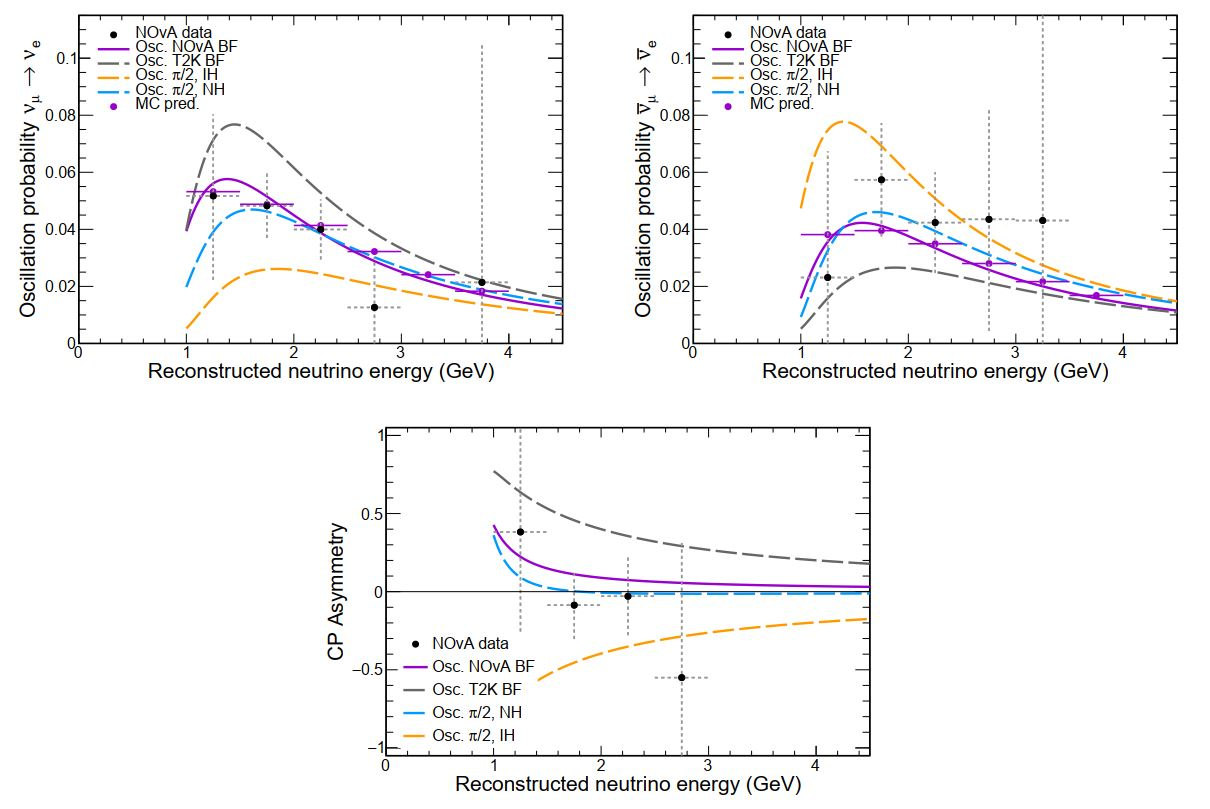
\includegraphics[scale=0.6]{Images/Liu_Result.JPG}
    \caption{Results based on NOvA data up to 2020}
    \label{Liu_result}
\end{figure}

\section{Bayesian and frequentist analysis}
\subsection{Concepts of Bayesian and frequentist approaches}
In Bayesian statistics, the interpretation of probability is more
general and includes degree of belief (called subjective probability). One can then speak of a probability density function (pdf)
for a parameter, which expresses one’s state of knowledge about
where its true value lies. Bayesian methods provide a natural
means to include additional information, which in general may be
subjective; in fact they require \textcolor{red}{prior probabilities} for the hypotheses (or parameters) in question, i.e. the degree of belief about the
parameters’ values, before carrying out the measurement. Using
Bayes’ theorem, the prior degree of belief is updated by the data from the experiment.

For example, we try to make an inference about a parameter $\mu$ whose true value $\mu_t$ is unknown. Assume that we do this by making a single measurement of an observable $x$ such that the probability density function (pdf) for obtaining the value $x$ depends on the
unknown parameter $\mu$ in a known way: we call this pdf $P(x|\mu)$. (Note that $x$ need not be a measurement of $\mu$; it just needs to be some observable whose pdf depends on $\mu$.) Now suppose a single measurement of $x$ yields $x_0$. We then get $P(x0|\mu)$ , known as the likelihood function, which usually denoted as $\mathcal{L}(x_0|\mu)$.
By applying  Bayes's Theorem, we get the “posterior” pdf $P(\nu_t|x_0)$:
\begin{equation}
\large
  P\left(\mu_t\vert x_0\right)=\frac{\mathcal L\left(x_0\vert\mu_t\right)P\left(\mu_t\right)}{P\left(x_0\right)}  
\end{equation}
Typically the denominator is just a normalization constant, so the major issue is what to use for $P(\mu_t)$, which is called the “prior” pdf. For the moment we assume that one has the prior pdf,  which is typically \textcolor{red}{subjective}.
There have been long-standing attempts to take the subjectivity out of the prior pdf, in order to have an “objective” Bayesian interval. However, the attempt to find a non-informative prior within Bayesian inference is
misguided. The real power of Bayesian inference lies in its ability to incorporate “informative” prior information, not “ignorance”. 

A Bayesian interval $[\mu_1, \mu_2]$ corresponding to a confidence level $\alpha$ can be constructed from the posterior pdf by requiring
\begin{equation}
\large
    \int_{\mu_1}^{\mu_2}P\left(\mu_t\vert x_0\right)\operatorname d\mu_t=\alpha
\end{equation}
These intervals are more properly called “ credible intervals”, although the phrase “Bayesian confidence intervals” is also used.

In frequentist statistics, probability is interpreted as the frequency of the outcome of a repeatable experiment. It is worth to note that one does not define a probability for a hypothesis or for the value of a parameter. In other words, no prior pdf is needed.

The unqualified phrase “confidence intervals” refers to frequentist intervals obtained with a procedure due to Neyman. A confidence interval like $[\mu_1, \mu_2]$ is a member of a set, such that the set has the property that
\begin{equation}
\large
    P\left(\mu\in\left[\mu_1,\;\mu_2\right]\right)=\alpha
\end{equation}
Here $\mu_1$ and $\mu_2$ are functions of the measured $x$, and the above equation refers to the varying confidence intervals $[\mu_1, \mu_2]$ from an ensemble of experiments with fixed $\mu_t$. For a set of confidence 
intervals [\textcolor{blue}{fig.\ref{confidenceBelt}}], the above equation is true for every allowed $\mu$. Thus, in particular, the intervals contain the fixed unknown $\mu_t$ in a fraction $\alpha$ of experiments. This is entirely different from the Bayesian
statement that the degree of belief that $\mu_t$ is in $[\mu_1, \mu_2]$ is $\alpha$.
\begin{figure}[]
    \centering
    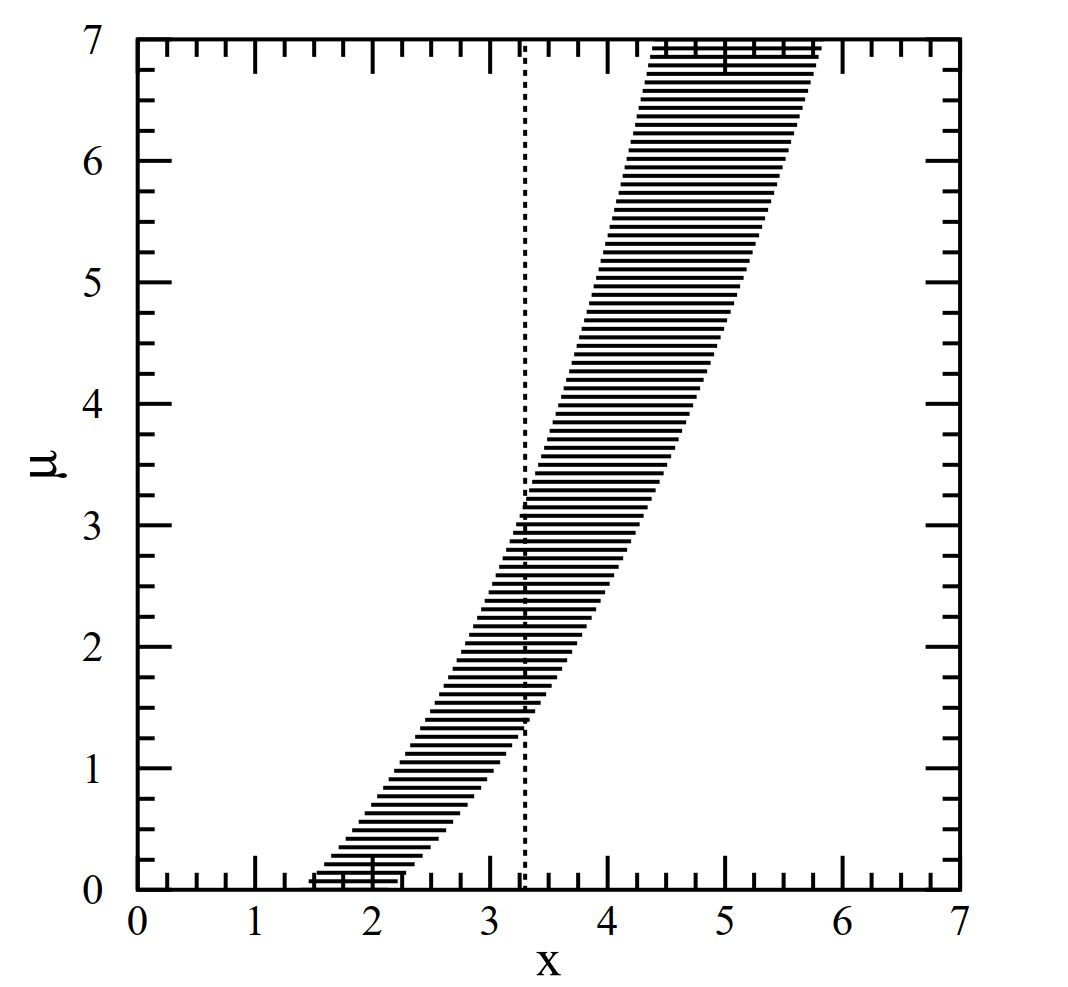
\includegraphics[scale=0.5]{Images/confidenceBand.JPG}
    \caption{A generic confidence belt construction and its use. For each value of $\mu$, one draws
a horizontal acceptance interval $\left[x_1,\;x_2\right]$ such that $P\left(\left.\left[x_1,\;x_2\right]\right|\mu\right)=\alpha$. 
Upon performing an experiment to measure $x$ and obtaining the value $x_0$, one draws the dashed vertical line through $x_0$. The confidence interval $\left[\mu_1,\;\mu_2\right]$ is the union of all values of $\mu$ for which the corresponding acceptance interval is intercepted by the vertical line.}
    \label{confidenceBelt}
\end{figure}

For more, refer to chapter 6 (P626) of \textit{$Review\; of\; Particle\; Physics$} by PDG, 2020:

\textcolor{blue}{$\href{https://pdg.lbl.gov/2021/html/computer_read.html}{https://pdg.lbl.gov/2021/html/computer\_read.html}$}

And \textit{A Unified Approach to the Classical
Statistical Analysis of Small Signals} by Feldman and Cousins:

\textcolor{blue}{$\href{https://arxiv.org/abs/physics/9711021v2}{https://arxiv.org/abs/physics/9711021v2}$}


\subsection{Data of NOvA}\label{cha22}
From the presentation of Liudmila 
$\footnote{\textcolor{blue}{\url{https://github.iu.edu/szh2/DUNE_Asymmetry/blob/ef67ef9353ff4a5fd7c1c715a429cadcb56e0430/papers/Acp.pdf}}}$, we can get some data from NOvA.

Like what are shown in the following figures, signals are made of three parts: Low PID, High PID and Peripheral, where the peripheral part is less reliable. Hence, only Low PID and High PID parts are considered. The left figure is the signal of neutrinos, while the right figure is for anti-neutrinos. 
\begin{figure}[H]
    \centering
    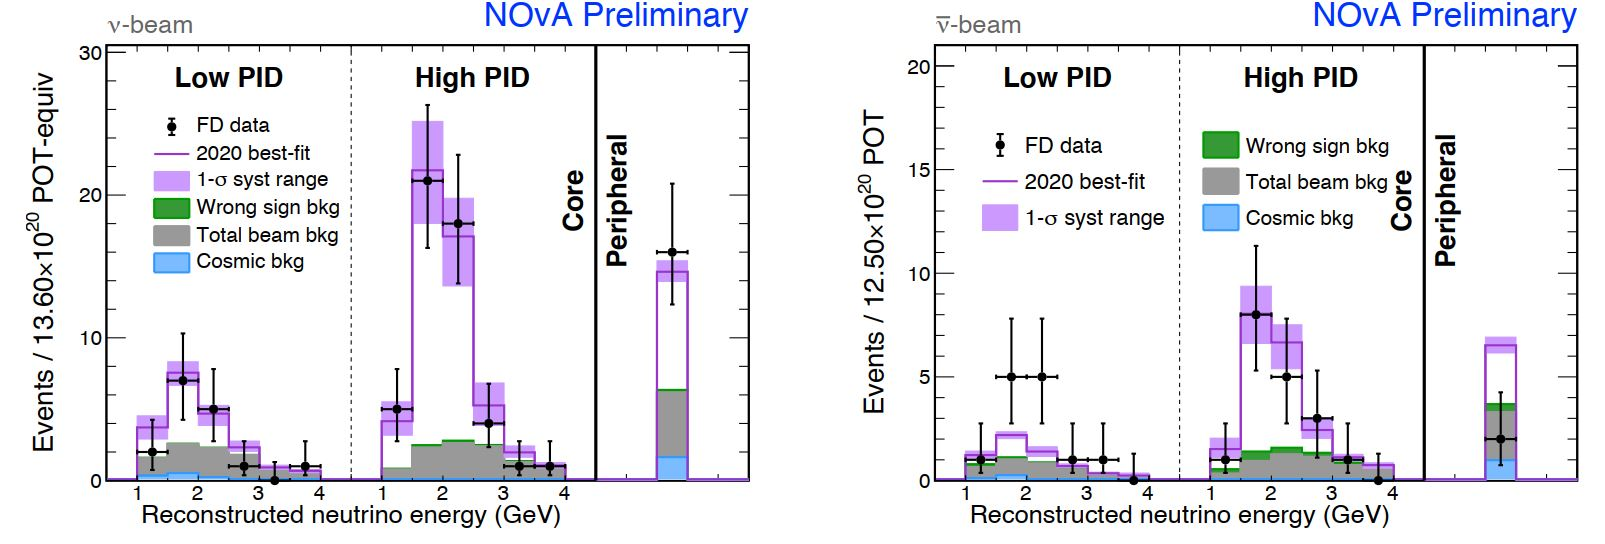
\includegraphics[scale=0.5]{Images/nominator.JPG}
    \caption{Measured Real Data "Signal"}
    \label{realData_1}
\end{figure}

If we combine signals and subtract related backgrounds, we will get \textcolor{blue}{fig.\ref{realData_2}}.
For upper two figures, they showed the real oscillated neutrino numbers. Here "FHC" refers to the neutrino mode of reaction and "RHC" is the anti-neutrino mode.
For lower left figure, it is the neutrino numbers if there is no oscillation; the lower right figure is results of anti-neutrino mode without oscillation. If we divide the results of upper two figures by those of lower two figures, the oscillation properties are obtained, which are top two figures in \textcolor{blue}{fig.$\ref{Liu_result}$}.


\begin{figure}[htbp]
    \centering
    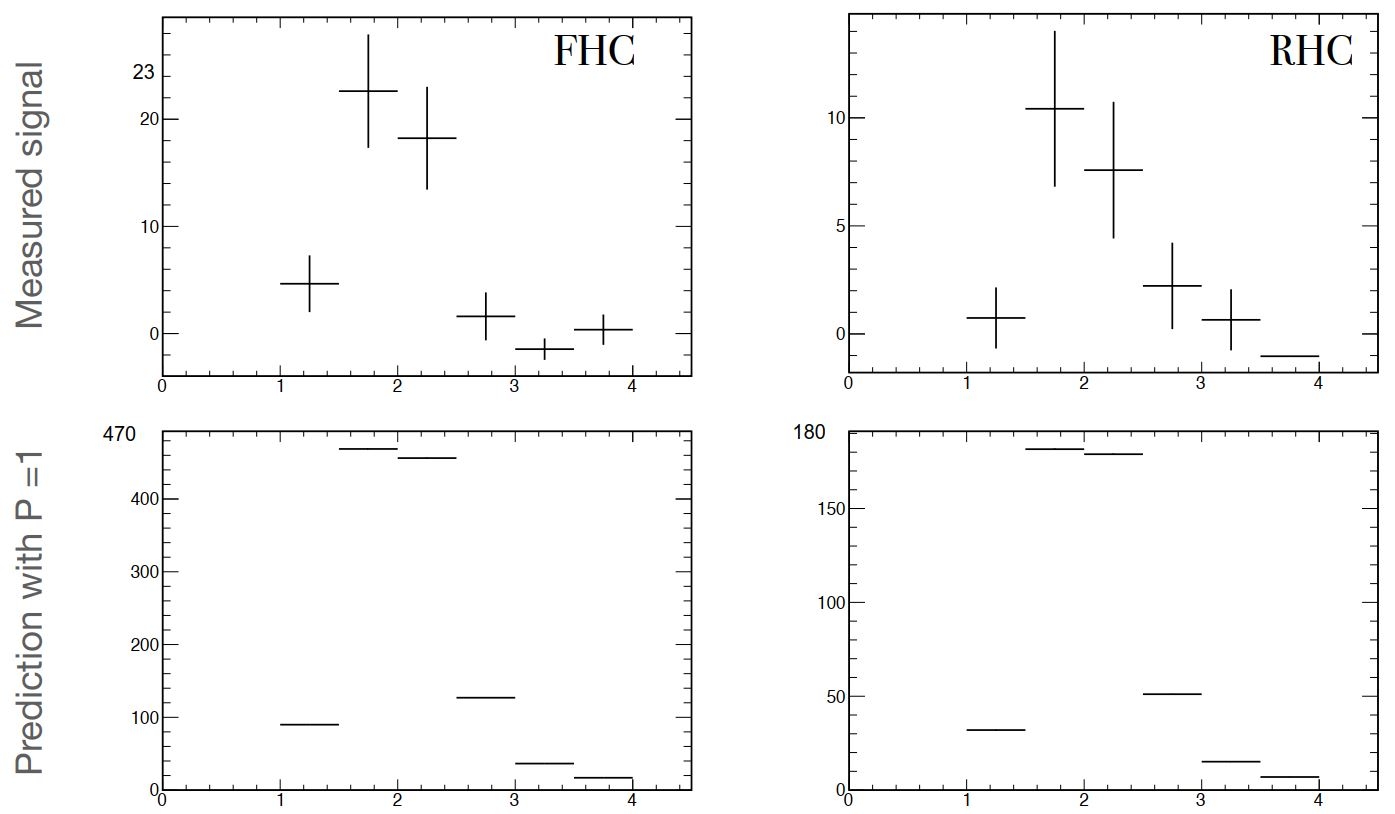
\includegraphics[scale=0.5]{Images/total.JPG}
    \caption{Signals subtracting the background}
    \label{realData_2}
\end{figure}
Taking the following formula
\begin{equation}
\large
    Asy=\frac{P\left(\nu_\mu\rightarrow\nu_e\right)-P\left({\overline\nu}_\mu\rightarrow{\overline\nu}_e\right)}{P\left(\nu_\mu\rightarrow\nu_e\right)+P\left({\overline\nu}_\mu\rightarrow{\overline\nu}_e\right)}
    \label{Asy_equ_1}
\end{equation}
The result of $A_{CP}$ (i.e. $Asy$) as a function of energy is reached [\textcolor{blue}{fig.$\ref{Liu_result}$}].
Liudmila showed that $A_{CP} = -0.0809091$ and the $68\%$ CL is $\left[-0.28212110,\;0.15234090\right]$ for 1.5GeV $\sim$ 2.0GeV range [\textcolor{blue}{fig.\ref{frequentistLiu}}].

\subsection{Frequentist approach in this analysis}
If we want to undergo the frquentist approach, we should construct the confidence belt [\textcolor{blue}{fig.\ref{confidenceBelt}}, here both $x$ and $\mu$ are $\delta_{CP}$] first. Just like what is shown in \textcolor{blue}{fig.$\ref{frequentistLiu}$} (from Liudmila's presentation
$\footnote{\textcolor{blue}{\url{https://github.iu.edu/szh2/DUNE_Asymmetry/blob/ef67ef9353ff4a5fd7c1c715a429cadcb56e0430/papers/acp_more_bins.pdf}}}$
), we set different initial values of $A_{CP}$, then get the analyzed results of $A_{CP}$ based on our analytical model, in which way we get the confidence belt. Finally, labeling the vertical line of real value of $A_{CP}$, we will finally get the confidence level.

\begin{figure}[htbp]
    \centering
    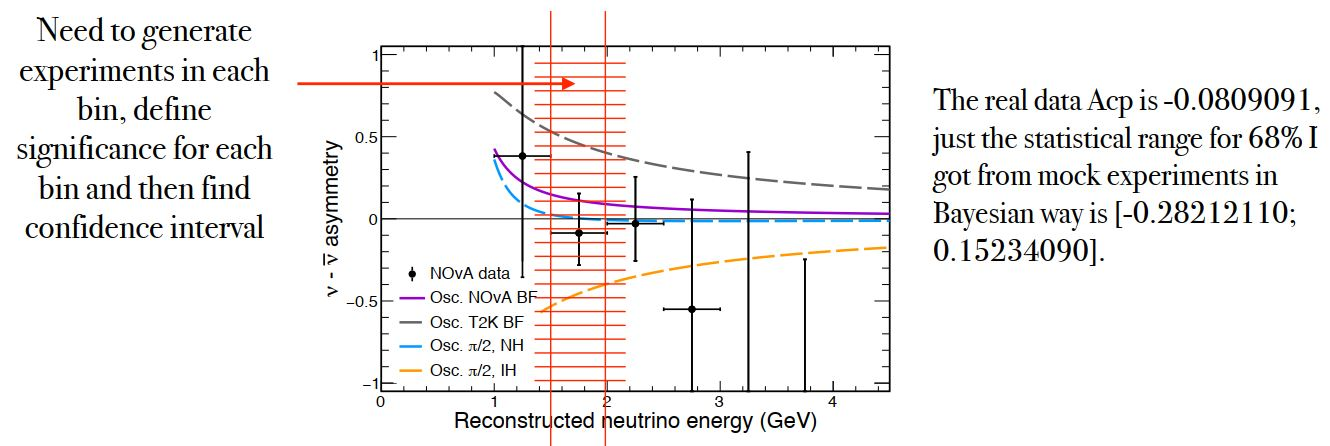
\includegraphics[width=13cm]{Images/onePointFive.JPG}
    \caption{frequentist explanations from Liudmila}
    \label{frequentistLiu}
\end{figure} 

For the process of neutrino oscillations, if the propagation distance and energy of neutrino flux are certain, the oscillation probability is solely the function of $\delta_{CP}$ after choosing certain values of mass ordering and oscillation angles $\theta_{13}$ and $\theta_{23}$. 
If there is no oscillation, the expected value of neutrinos and anti-neutrinos are certain, just like the lower two figures of \textcolor{blue}{fig.\ref{realData_2}}.
Hence, if all other variables are certain, the number of neutrinos and anti-neutrinos generated from oscillation are functions of $\delta_{CP}$, i.e. $n_\nu=n_\nu\left(\delta_{CP}\right),\;n_{\overline\nu}=n_{\overline\nu}\left(\delta_{CP}\right)$. Hence, for certain value of $\delta_{CP}$, the relation between $n_\nu$ and $n_{\overline\nu}$ is certain. 

According to the calculation formula of $Asy$ [\textcolor{blue}{equ.\ref{Asy_equ_1}}], there are different ways to change the value of $A_{CP}$. For example, we could keep one of $P\left({\overline\nu}_\mu \rightarrow {\overline\nu}_e\right)$ and $P\left(\nu_\mu \rightarrow \nu_e\right)$ invariant and change another of them each time. From last paragraph we know there exists a constraint for number of neutrinos and anti-neutrinos.

For simplicity, here I keep the sum of neutrinos and anti-neutrinos invariant and change number of neutrinos each time so as to set different values of $A_{CP}$. Consequently, different asymmetry values correspond to different points in the red line of \textcolor{blue}{fig.\ref{constraint}}. 

\begin{figure}[htbp]
    \centering
    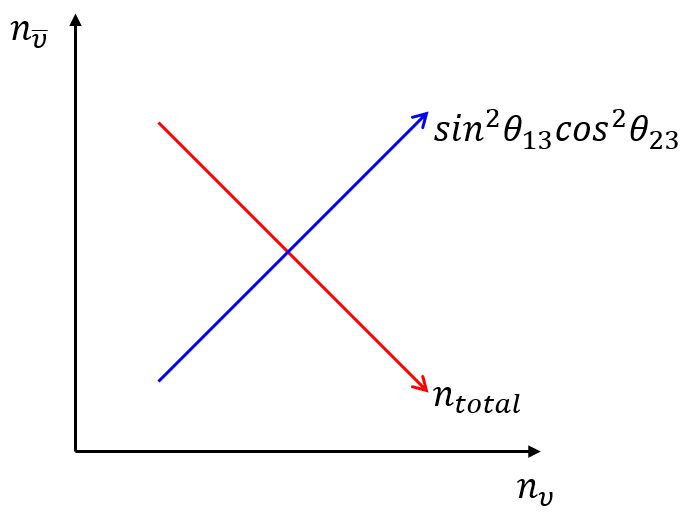
\includegraphics[width=10cm]{Images/axis.png}
    \caption{Constraint on number of neutrinos and number of anti-neutrinos}
    \label{constraint}
\end{figure} 


\section{Simulations}
When the number of neutrinos is small, it obeys the Poisson distribution. Hence in my simulation, I used two Poisson distributions to generate neutrinos and anti-neutrinos.  

To make the simulation process more clear, I splitted it into two steps. The first step is the exploration of two Poisson distributions; the second step simulated the case closer to the real condition, i.e. considering the background of neutrinos and anti-neutrinos.

\subsection{Pure mathematical simulation without background}
\subsubsection{Illustration of the simulation}
For these two Poisson distributions, the mean values of them are number of neutrinos and anti-neutrinos respectively. The randomly generated neutrinos and anti-neutrinos obey the following equation:
\begin{equation}
\large
    \left\{\begin{array}{l}N_\nu\sim P\left(n_\nu,\;N_\nu\right)=\frac{\left(n_\nu\right)^{N_\nu}}{N_\nu!}e^{-n_\nu}\\\\N_{\overline\nu}\sim P\left(n_{\overline\nu},\;N_{\overline\nu}\right)=\frac{\left(n_{\overline\nu}\right)^{N_{\overline\nu}}}{N_{\overline\nu}!}e^{-n_{\overline\nu}}\end{array}\right.
\end{equation}

The total number of neutrinos and anti-neutrinos are 34. The number of neutrinos without oscillation is taken as 480; the number of anti-neutrinos without oscillation is taken as 170. 

During this step, I changed the initial number of neutrinos so as to set different values of $A_{CP}$ (i.e. $Asy$ in the following expression). For example, if the number of neutrinos is 7.98 (since it is the mean value of the distribution, it is not necessarily be an integer.), then we get:
\begin{equation}
\large
    Asy=\frac{\frac{7.98}{480}-\frac{26.02}{170}}{\frac{7.98}{480}-\frac{26.02}{170}}=-0.800
    \label{asy_real}
\end{equation}
During my simulation, $A_{CP}$ is set as $-0.8,\;-0.7,\;-0.6,\;...0.6,\;0.7,\;0.8$. For each value of $A_{CP}$, the simulation is repeated for $10^6$ times, i.e. each Poisson generator worked for $10^6$ times.   


\subsubsection{Results of the simulation}
\textcolor{blue}{fig.\ref{figs_noBKG}} showed parts of the simulations. We can find that the distribution become wider and wider as the initial value of $Asy$ becomes larger and larger.

\begin{figure}[htbp]
\centering
\subfigure[$Asy=-0.8$]{
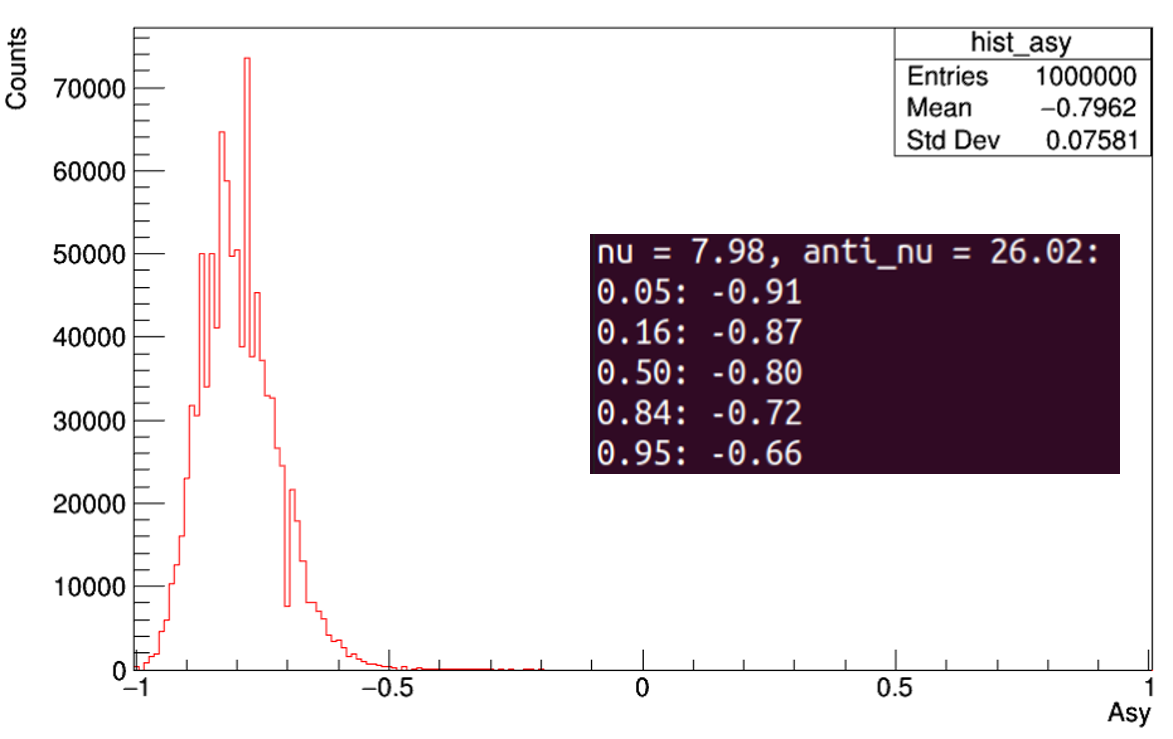
\includegraphics[width=4.2cm]{Images/Asy_n8_noBKG.png}
%\caption{fig1}
}
\quad
\subfigure[$Asy=-0.5$]{
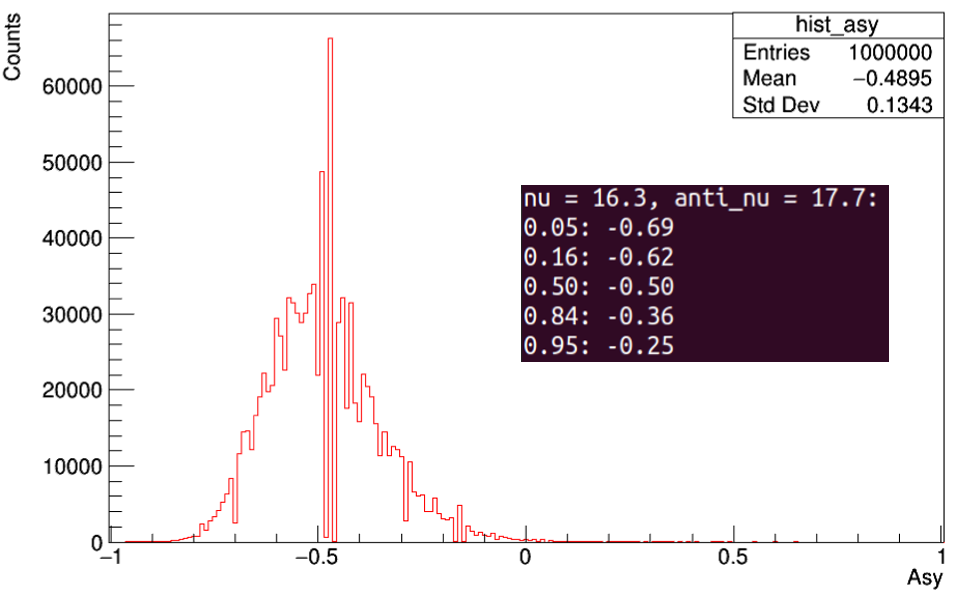
\includegraphics[width=4.2cm]{Images/Asy_n5_noBKG.png}
}
\quad
\subfigure[$Asy=-0.2$]{
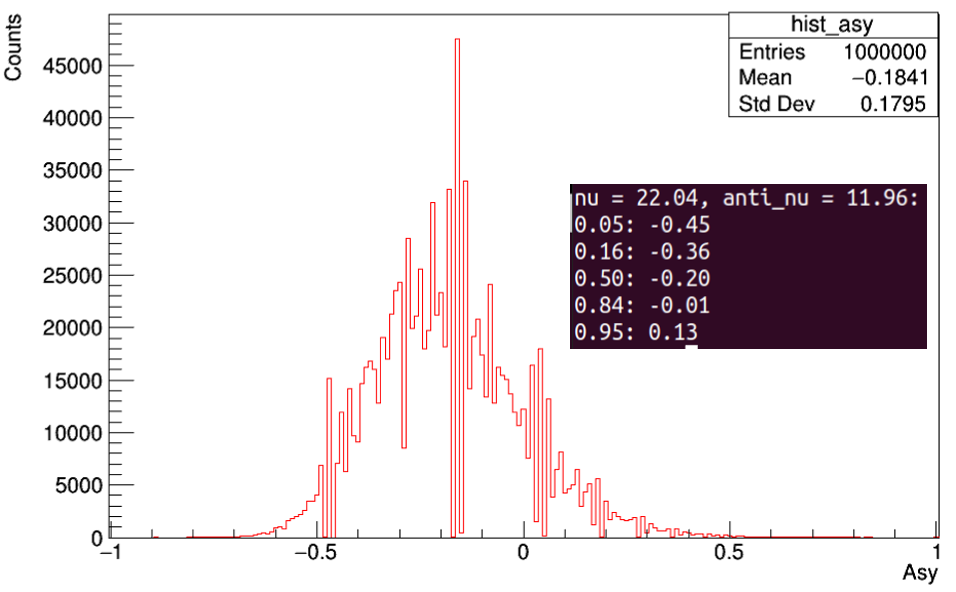
\includegraphics[width=4.2cm]{Images/Asy_n2_noBKG.png}
}
\quad
\subfigure[$Asy=+0.2$]{
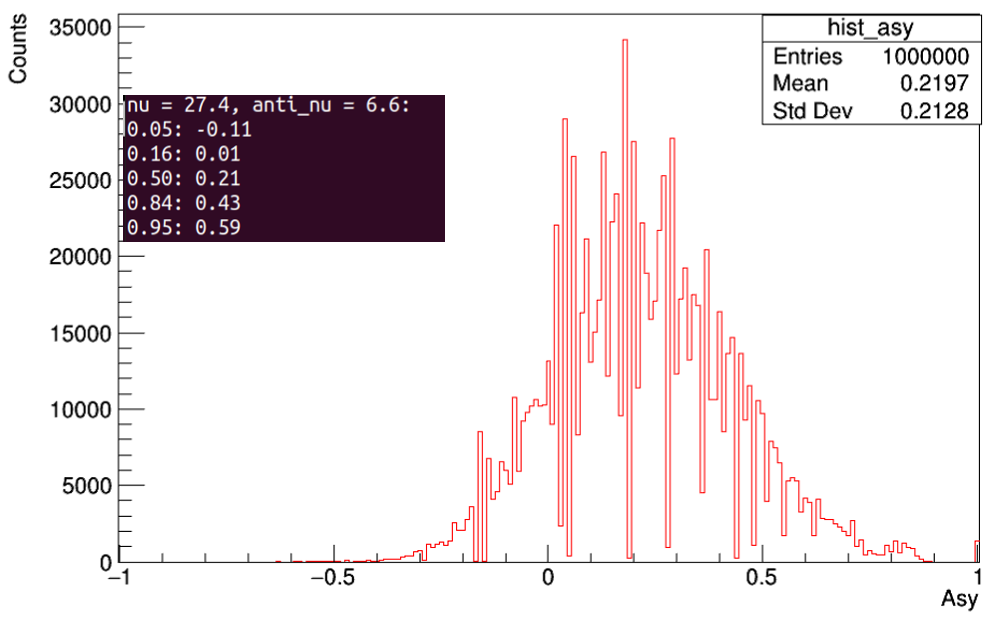
\includegraphics[width=4.2cm]{Images/Asy_p2_noBKG.png}
}
\quad
\subfigure[$Asy=+0.5$]{
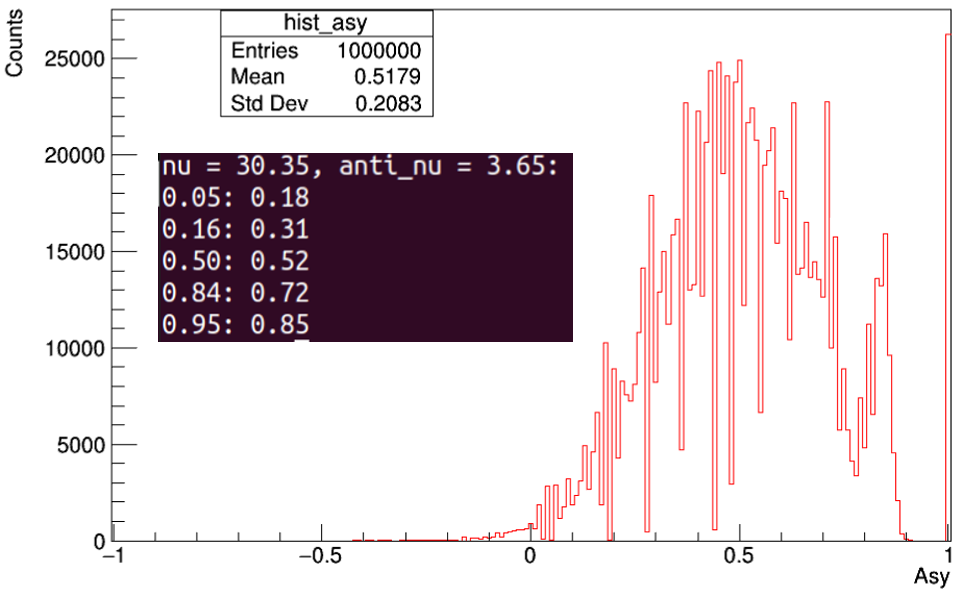
\includegraphics[width=4.2cm]{Images/Asy_p5_noBKG.png}
}
\quad
\subfigure[$Asy=+0.8$]{
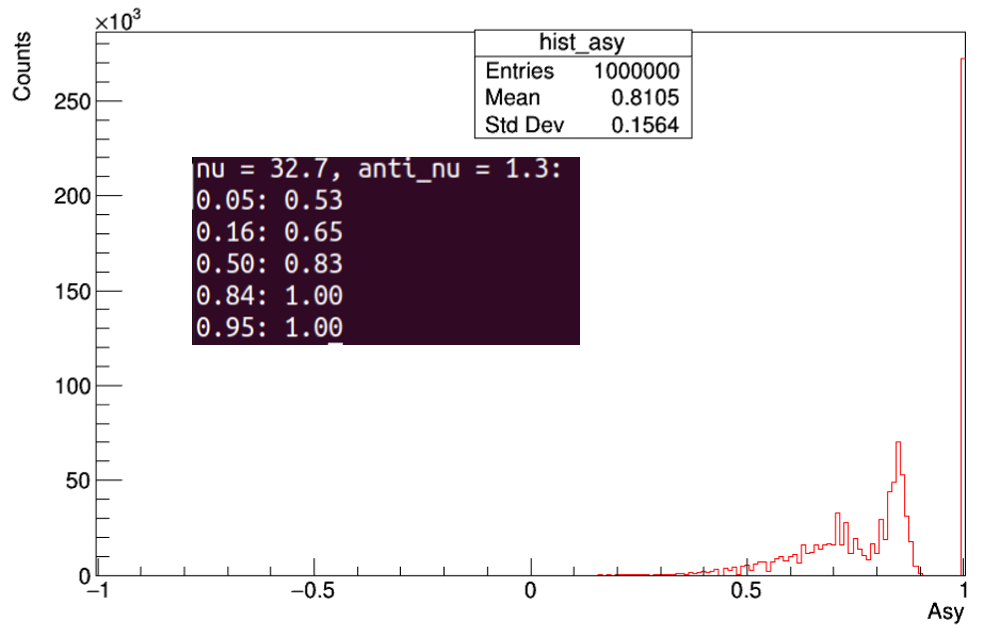
\includegraphics[width=4.2cm]{Images/Asy_p8_noBKG.png}
}
\caption{Parts of the distribution of $A_{CP}$ for different set values of $A_{CP}$.}
\label{figs_noBKG}
\end{figure}

\textcolor{blue}{fig.\ref{figure_dis_noBKG}} showed the distribution of the whole simulations. We can find that mean values of the simulation agree well with the initial set of asymmetry values; the standard deviation becomes larger then smaller as the initial value of asymmetry moves from $-0.8$ to $+0.8$.
\begin{figure}[htbp]
    \centering
    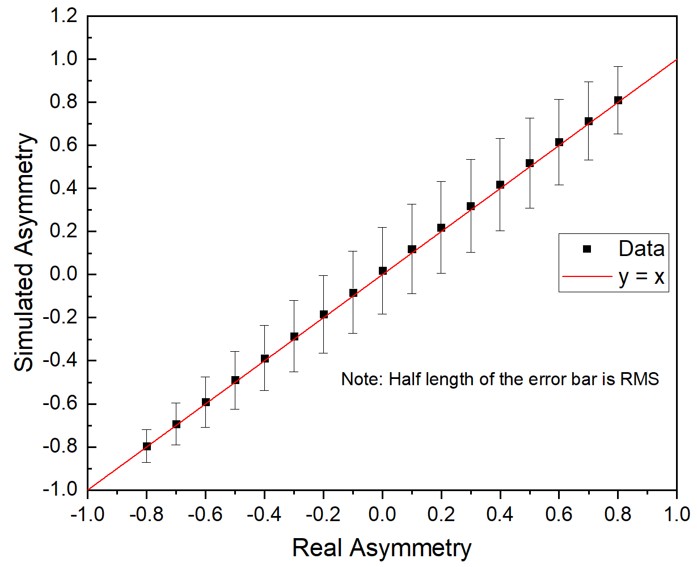
\includegraphics[width=10cm]{Images/full_noBKG.png}
    \caption{Data points here are the results of the simulation; related error bar corresponds to the standard deviation value for each distribution in \textcolor{blue}{fig.\ref{figs_noBKG}}}
    \label{figure_dis_noBKG}
\end{figure} 

For more information, refer to \textcolor{blue}{fig.\ref{parts_noBKG}}.


\subsection{Simulation with background}
\subsubsection{Illustration of the process}
After finishing the simple simulation of two Poisson distributions, I tried to simulate the case which is closer to the real condition.

Focusing on the 1.5 GeV $\sim$ 2.0 GeV range, it is easy to find that [\textcolor{blue}{fig.\ref{Liu_result}}] the data is what is shown in the following table:
\begin{table}[H]
\begin{tabular}{cccccc}
\hline
\multicolumn{1}{|c|}{}                                                             & \multicolumn{1}{c|}{\begin{tabular}[c]{@{}c@{}}High PID\\ Event\end{tabular}} & \multicolumn{1}{c|}{\begin{tabular}[c]{@{}c@{}}High PID\\ Background\end{tabular}} & \multicolumn{1}{c|}{\begin{tabular}[c]{@{}c@{}}Low PID\\ Event\end{tabular}} & \multicolumn{1}{c|}{\begin{tabular}[c]{@{}c@{}}Low PID\\ Background\end{tabular}} & \multicolumn{1}{c|}{\begin{tabular}[c]{@{}c@{}}Prediction \\ with P=1\end{tabular}} \\ \hline
\multicolumn{1}{|c|}{\begin{tabular}[c]{@{}c@{}}Neutrino\\ Mode\end{tabular}}      & \multicolumn{1}{c|}{21}                                                       & \multicolumn{1}{c|}{2.5}                                                           & \multicolumn{1}{c|}{7}                                                       & \multicolumn{1}{c|}{2.5}                                                          & \multicolumn{1}{c|}{470}                                                            \\ \hline
\multicolumn{1}{|c|}{\begin{tabular}[c]{@{}c@{}}Anti-neutrino\\ Mode\end{tabular}} & \multicolumn{1}{c|}{8}                                                        & \multicolumn{1}{c|}{1.25}                                                          & \multicolumn{1}{c|}{5}                                                       & \multicolumn{1}{c|}{1.25}                                                         & \multicolumn{1}{c|}{180}                                                            \\ \hline
\multicolumn{1}{l}{}                                                               & \multicolumn{1}{l}{}                                                          & \multicolumn{1}{l}{}                                                               & \multicolumn{1}{l}{}                                                         & \multicolumn{1}{l}{}                                                              & \multicolumn{1}{l}{} \end{tabular}
\caption{Data for neutrinos and anti-neutrinos}
\label{data_table}
\end{table}

The formula to calculate the asymmetry is as follows:
\begin{equation}
    \large
    Asy=\frac{\frac{n_\nu}{n_{\nu\_pred}}-\frac{n_{\overline\nu}}{n_{\overline\nu\_pred}}}{\frac{n_\nu}{n_{\nu\_pred}}+\frac{n_{\overline\nu}}{n_{\overline\nu\_pred}}}
\end{equation}
This formula is just the same as \textcolor{blue}{equ.$\ref{Asy_equ_1}$}.
All of the quantities in above equation contain both low PID and high PID data.
$n_\nu$ here is the number of neutrinos; $n_{\overline\nu}$ is the number of anti-neutrinos; $n_{\nu\_pred}$ is the number of nuetrinos without oscillation; $n_{\overline\nu\_pred}$ is the number of anti-neutrinos without oscillation. From above table we know
\begin{equation}
\large
    \left\{\begin{array}{l}n_\nu+n_{\overline\nu}=28+13-5-2.5=33.5\\n_{\nu\_pred}=470;\;\;\;n_{\overline\nu\_pred}=180\end{array}\right.
\end{equation}
Initially $n_\nu=21+7-5=23$ and $n_{\overline\nu}=8+5-2.5=10.5$, we can get that
\begin{equation}
\large
    Asy=\frac{\frac{23}{470}-\frac{10.5}{180}}{\frac{23}{470}+\frac{10.5}{180}}=-0.087
    \label{asy_cal_1}
\end{equation}
The error corresponding to the real data value (0.081) is smaller than $10\%$. Hence the data in above table is fairly reasonable.

Since we are taking the frequentist approach here, only $n_\nu+n_{\overline\nu}=33.5$ is required in our process when building the confidence belt. I will only change the value of $n_\nu$ to set different values of $A_{CP}$.

The following is the process of the simulation:

The number of neutrinos $N_\nu$ and anti-neutrinos $N_{\overline\nu}$ obey the following distributions, where $n_{n_{\nu\_bkg}}=5$ and $n_{n_{\overline\nu\_bkg}}=2.5$ are the background of neutrinos and anti-neutrinos respectively. We can find their values in \textcolor{blue}{table.\ref{data_table}}.
\begin{equation}
\large
    \left\{\begin{array}{l}N_\nu\sim P\left(n_\nu+n_{\nu\_bkg},\;N_\nu\right)=\frac{\left(n_\nu+n_{\nu\_bkg}\right)^{N_\nu}}{N_\nu!}e^{-\left(n_\nu+n_{\nu\_bkg}\right)}\\N_{\overline\nu}\sim P\left(n_{\overline\nu}+n_{\overline\nu\_bkg},\;N_{\overline\nu}\right)=\frac{\left(n_{\overline\nu}+n_{\overline\nu\_bkg}\right)^{N_{\overline\nu}}}{N_{\overline\nu}!}e^{-\left(n_{\overline\nu}+n_{\overline\nu\_bkg}\right)}\end{array}\right.
    \label{generator_bkg}
\end{equation}

After generating the number of neutrinos and anti-neutrinos, we can use the following expression to get the simulated value of asymmetry:
\begin{equation}
\large
    Asy_{simu}=\frac{{\frac{N_\nu-n_{\nu\_bkg}}{n_{\nu\_pred}}}-\frac{N_{\overline\nu}-n_{\overline\nu\_bkg}}{n_{\nu\_pred}}}{\frac{N_\nu-n_{\nu\_bkg}}{n_{\nu\_pred}}+\frac{N_{\overline\nu}-n_{\overline\nu\_bkg}}{n_{\overline\nu\_pred}}}
    \label{calculating_Asy}
\end{equation}
From \textcolor{blue}{equ.\ref{generator_bkg}} we know the numbers generated contain the background. Hence we need subtract the background when calculating the asymmetry in \textcolor{blue}{equ.\ref{calculating_Asy}}.

\subsubsection{Result}
Parts of the simulated results are as follows:
\begin{figure}[H]
\centering
\subfigure[Asy=-0.8]{
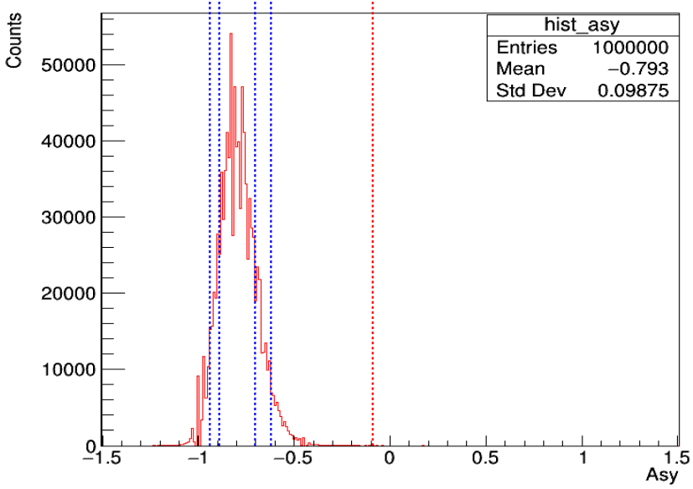
\includegraphics[width=4.2cm]{Images/bg_n8.png}
%\caption{fig1}
}
\quad
\subfigure[Asy=-0.4]{
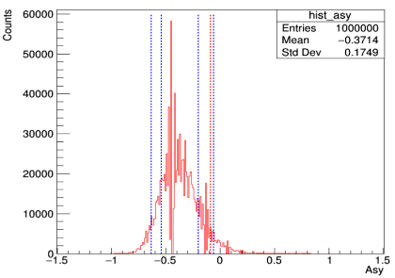
\includegraphics[width=4.2cm]{Images/bg_n4.png}
}
\quad
\subfigure[Asy=-0.1]{
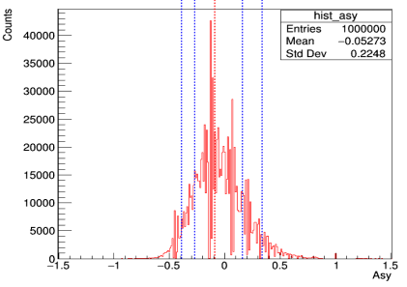
\includegraphics[width=4.2cm]{Images/bk_n1.png}
}
\quad
\subfigure[Asy=+0.1]{
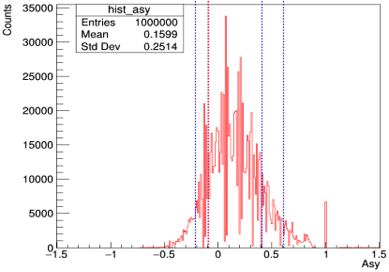
\includegraphics[width=4.2cm]{Images/bk_p1.png}
}
\quad
\subfigure[Asy=+0.4]{
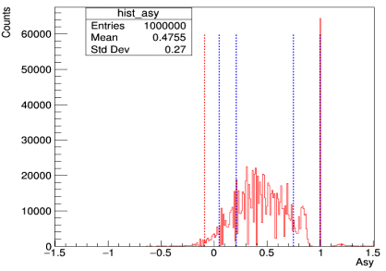
\includegraphics[width=4.2cm]{Images/bk_p4.png}
}
\quad
\subfigure[Asy=+0.8]{
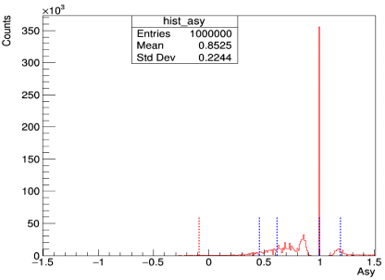
\includegraphics[width=4.2cm]{Images/bk_p8.png}
}
\caption{Parts of the results. In each figure, there are four blue dashed lines, which represent the 5\%, 16\%, 84\% point for the integral of the distribution. The red dashed line is $Asy=-0.087$, the value calculated in \textcolor{blue}{equ.\ref{asy_cal_1}}.}
\label{multi_figures_bkg}
\end{figure}
We can find that there are some distributions beyond $Asy=+1.0$, which is impossible in the case of no background.

The statistical results are shown in \textcolor{blue}{fig.\ref{final_result_bkg}}.
We find the bias between the simulated asymmetry value and the initial set of asymmetry becomes apparent since the initial set value of Asy is larger than zero. It is also apparent that the standard deviation becomes larger when the initial set of asymmetry value becomes larger.
\begin{figure}[H]
    \centering
    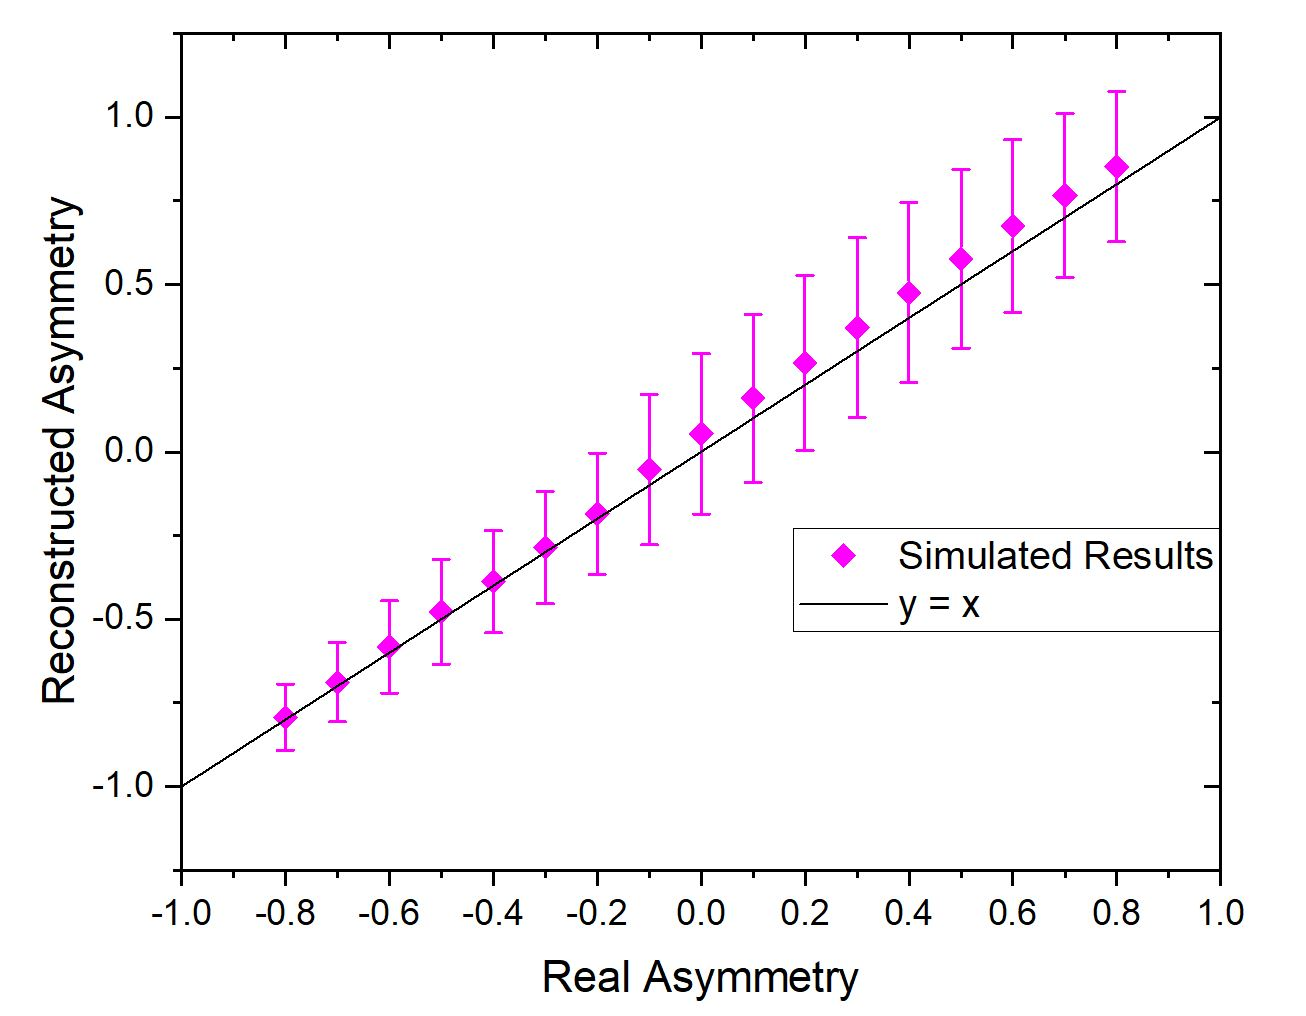
\includegraphics[width=12cm]{Images/distribution_bkg.JPG}
    \caption{Results of all simulations. 
“Real Asymmetry” here refers to the initial set value of asymmetry, while “Reconstructed Asymmetry” refers to the simulated value of asymmetry. The purple rhombus are the mean value of each distribution shown in \textcolor{blue}{fig.\ref{multi_figures_bkg}}. The error bar is the standard deviation of the distribution.}
    \label{final_result_bkg}
\end{figure} 
This can be initially explained by the statistical fluctuations of $N_\nu$ and $N_{\overline\nu}$. Since $P\left(\nu_\mu\rightarrow\nu_e\right)=\frac{n_\nu}{n_{\nu\_pred}},\;P\left({\overline\nu}_\mu\rightarrow{\overline\nu}_e\right)=\frac{\displaystyle n_{\overline\nu}}{\displaystyle n_{\overline\nu\_pred}}$ as well as $\frac{\displaystyle n_{\nu\_pred}}{\displaystyle n_{\overline\nu\_pred}}=\frac{\displaystyle470}{\displaystyle180}\approx3$, 
from \textcolor{blue}{equ.\ref{Asy_equ_1}} we can get:
\begin{equation}
\large
    \frac{d\left(Asy\right)}{Asy}\propto\left\{\frac{2\cdot\left(3n_{\overline\nu}\right)}{\left(n_\nu^2-\left(3n_{\overline\nu}\right)^2\right)}dn_\nu-\frac{2\cdot n_\nu}{\left(n_\nu^2-\left(3n_{\overline\nu}\right)^2\right)}d\left(3n_{\overline\nu}\right)\right\}
\end{equation}
Since the standard deviation of Poisson distribution equals to the mean value, we will have:
\begin{equation}
    \large
    \triangle\left(Asy\right)\propto\frac{Asy\cdot\left(3n_{\overline\nu}\right)\cdot n_\nu}{\left(n_\nu^2-\left(3n_{\overline\nu}\right)^2\right)}
\end{equation}
For $Asy=-0.8$, after refering \textcolor{blue}{fig.\ref{table_BKG}}, we get $\triangle\left(Asy\right)\sim0.08C$, where $C$ is the constant proportionality coefficient.

Similarly, for $Asy=+0.1$, we get $\triangle\left(Asy\right)\sim0.82C$;

For $Asy=+0.6$, we get $\triangle\left(Asy\right)\sim0.3C$.

More details about the standard deviation and difference between simulated value and initial set value of asymmetry are shown in \textcolor{blue}{fig.\ref{details_std}}.
\begin{figure}[htbp]
\centering
\subfigure[Standard Deviation]{
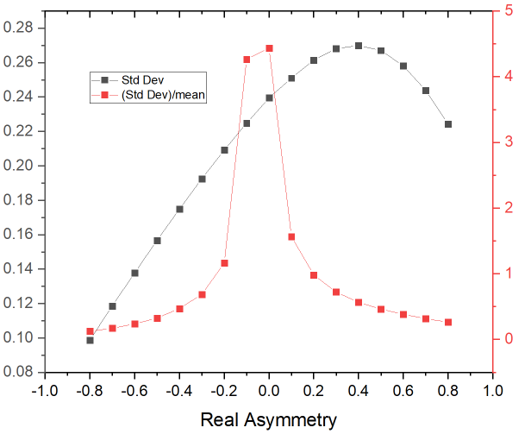
\includegraphics[width=6cm]{Images/bkg_std_1.png}
%\caption{fig1}
}
\quad
\subfigure[Bias]{
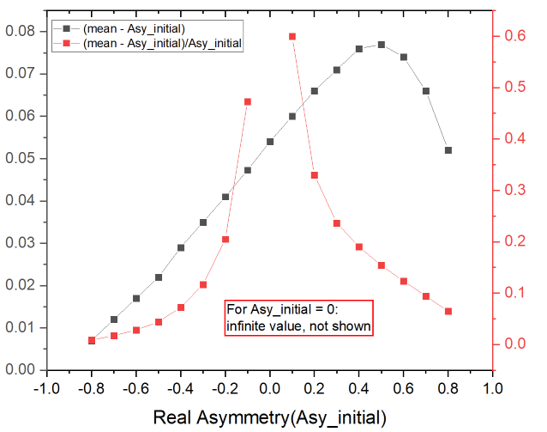
\includegraphics[width=6cm]{Images/bkg_std_2.png}
}
\caption{The left is the distribution of standard deviation of each simulations; The right is the difference between the simulated asymmetry and the initial set asymmetry.}
\label{details_std}
\end{figure}

According to \textcolor{blue}{Sec.\ref{cha22}}, we know  $A_{CP} = -0.0809091$ and the $68\%$ confidence level is $\left[-0.28212110,\;0.15234090\right]$ of 1.5GeV $\sim$ 2.0GeV range for Bayesian approach. 

If the results under Bayesian approach coincide with those under frequentist approach, we would expect the real value is close to the 84\% point if we set the initial value of asymmetry as $-0.28212110$, i.e. the left one sigma boundary of the Bayesian approach. It is also expected that the real value is close to the 16\% point if we set the initial value of asymmetry as $0.15234090$.  

\begin{figure}[H]
    \centering
    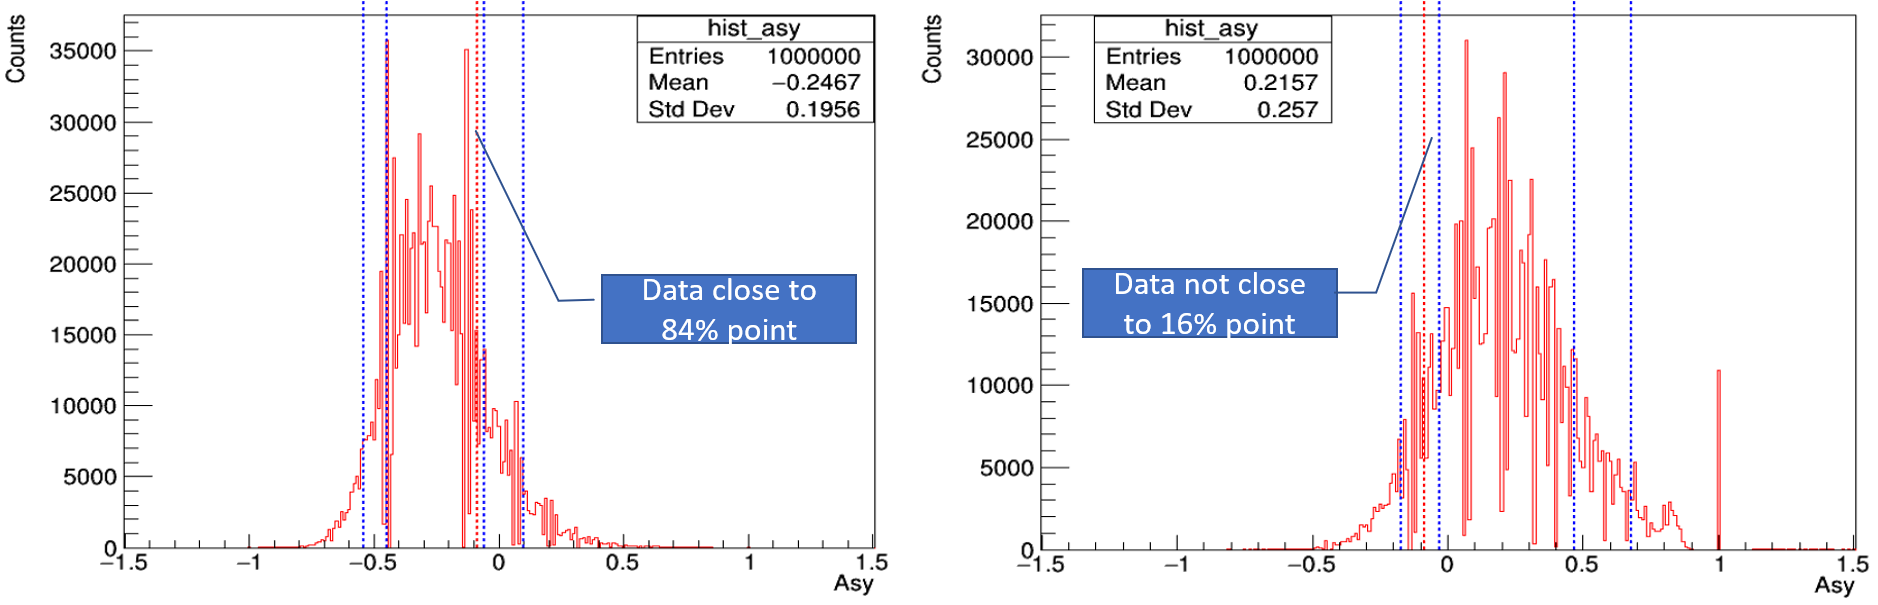
\includegraphics[width=12cm]{Images/nearRange.png}
    \caption{For the left figure, the initial set of asymmetry is $-0.282$; For the right figure, the initial value of asymmetry is $+0.152$.}
    \label{twoRanges}
\end{figure} 

Consequently, the red dashed line is expected to coincide with the third blue line for the left figure of \textcolor{blue}{fig.\ref{twoRanges}}; while the red dashed line is expected to coincide with the second blue line for the right figure. Unfortunately, we find that those two lines do not coincide with each other well for above right figure.

\section{Conclusion}
Based on the analytical model of NOvA, Liudmila also made the analysis
$\footnote{\textcolor{blue}{\url{https://github.iu.edu/szh2/DUNE_Asymmetry/blob/ef67ef9353ff4a5fd7c1c715a429cadcb56e0430/papers/acp_more_bins.pdf}}}$
under frequentist approach.
She showed that the one sigma region is approximate to $\left[-0.4,\;0.2\right]$. We know the region is $\left[-0.28212110,\;0.15234090\right]$ under Bayesian approach. Moreover, the consistence between the median value and the initial set value of asymmetry is bad.

Under my analysis, the one sigma region is approximate
$\footnote{This is because I only set finite discrete values of asymmetry when doing this simulation.}$
to $\left[-0.3,\;0.1\right]$ (refer to the confidence belt in \textcolor{blue}{fig.\ref{final_result_bkg}} and data in \textcolor{blue}{fig.\ref{table_BKG}}). Similarly, the consistence between the median value and the initial set value of asymmetry in my analysis is bad, either [\textcolor{blue}{fig.\ref{table_BKG}}].  

We can initially conclude that result under frequentist approach does not coincide well with result under Bayesian approach.

It is not reasonable to say that my analysis got a better result compared to that of Liudmila for the fact that my region is closer to the region of Bayesian approach. 
On one hand, the closer the region gotten from frequentist approach is to the region of the Bayesian approach, the stronger the consistence of these two approach is. On the other hand, my analysis is a purely mathematical exploration based on the fluctuation properties of Poisson distribution, while Liudmila's analysis considered the physical model provided by NOvA, which is more reasonable.

At last, I hope this analysis will be inspiring for the exploration of asymmetry.
 


\newpage
\section{Backup}
\begin{figure}[H]
\begin{minipage}[t]{0.25\linewidth}
\centering
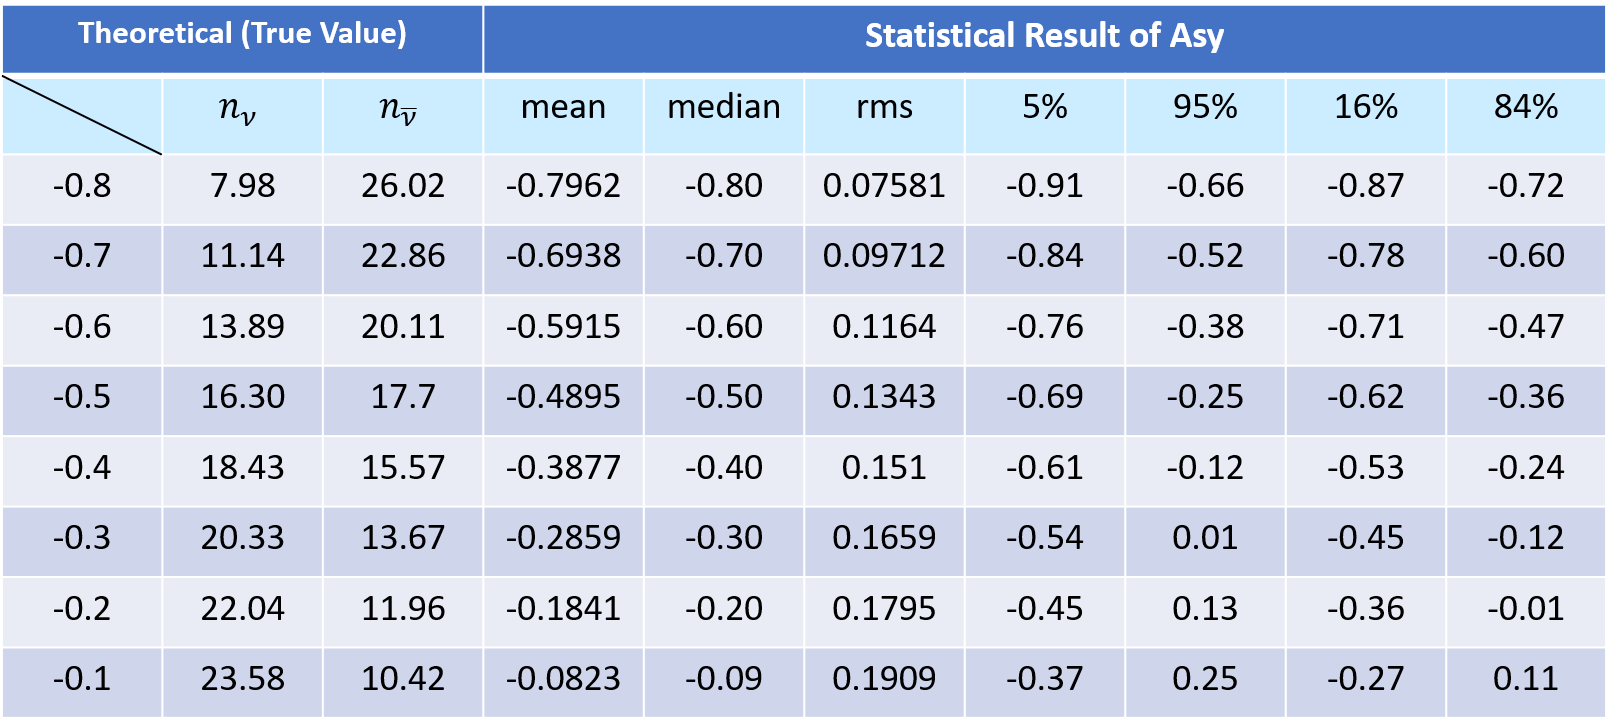
\includegraphics[width=5.5in]{Images/table_noBKG.png}
\end{minipage}%

\begin{minipage}[t]{0.25\linewidth}
\centering
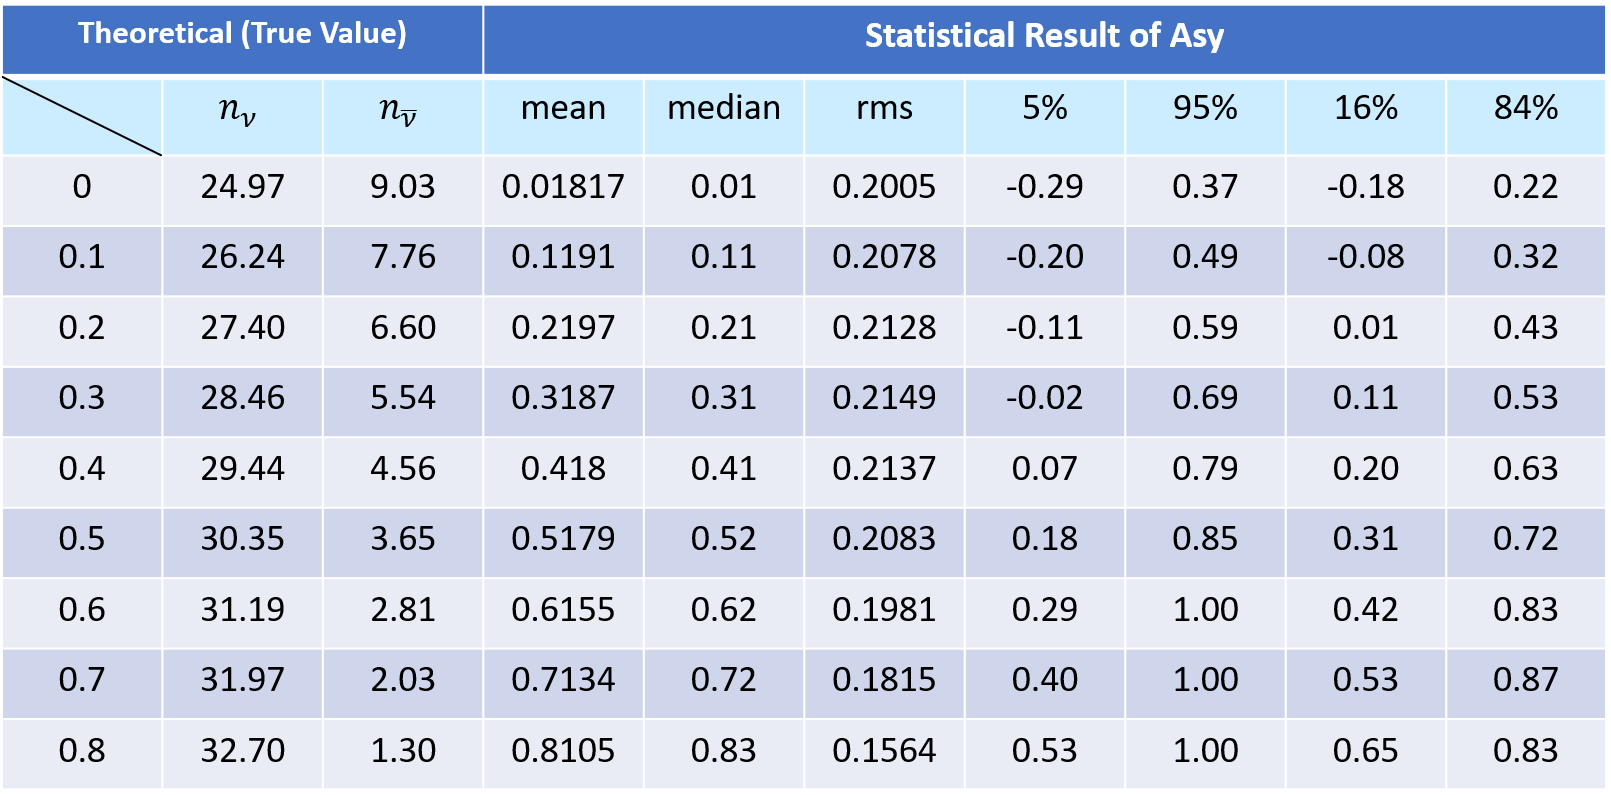
\includegraphics[width=5.5in]{Images/table_noBKG_2.png}
\end{minipage}%
\caption{ Statistical result without background. Here “Theoretical” refers to the initial values we set for the simulation; “Statistical” are the simulated results.}
\label{parts_noBKG}
\end{figure}





\newpage
\begin{figure}[H]
\begin{minipage}[t]{0.25\linewidth}
\centering
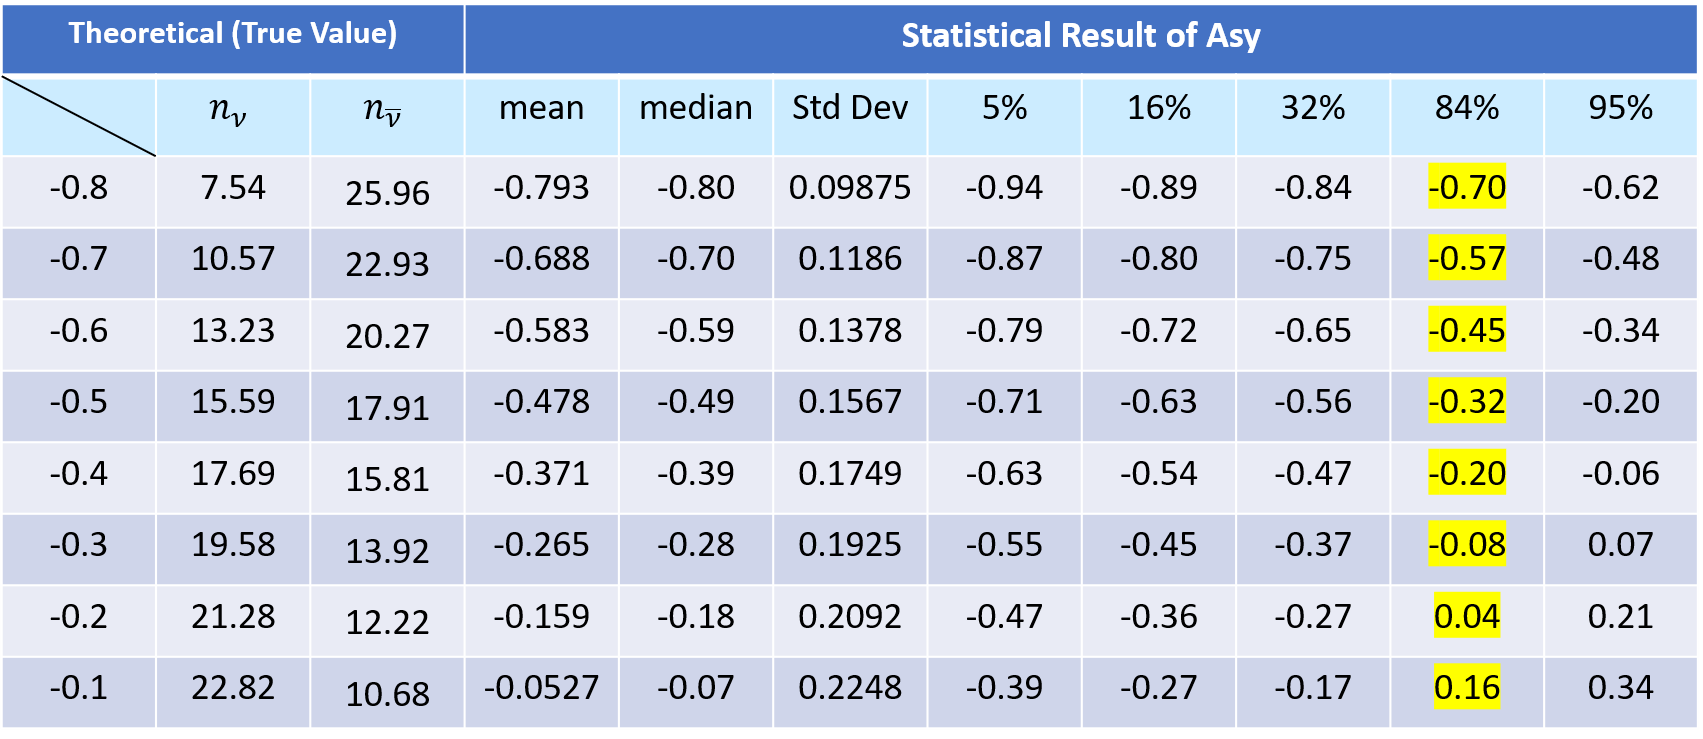
\includegraphics[width=5.5in]{Images/table_bkg_1.png}
\end{minipage}%

\begin{minipage}[t]{0.25\linewidth}
\centering
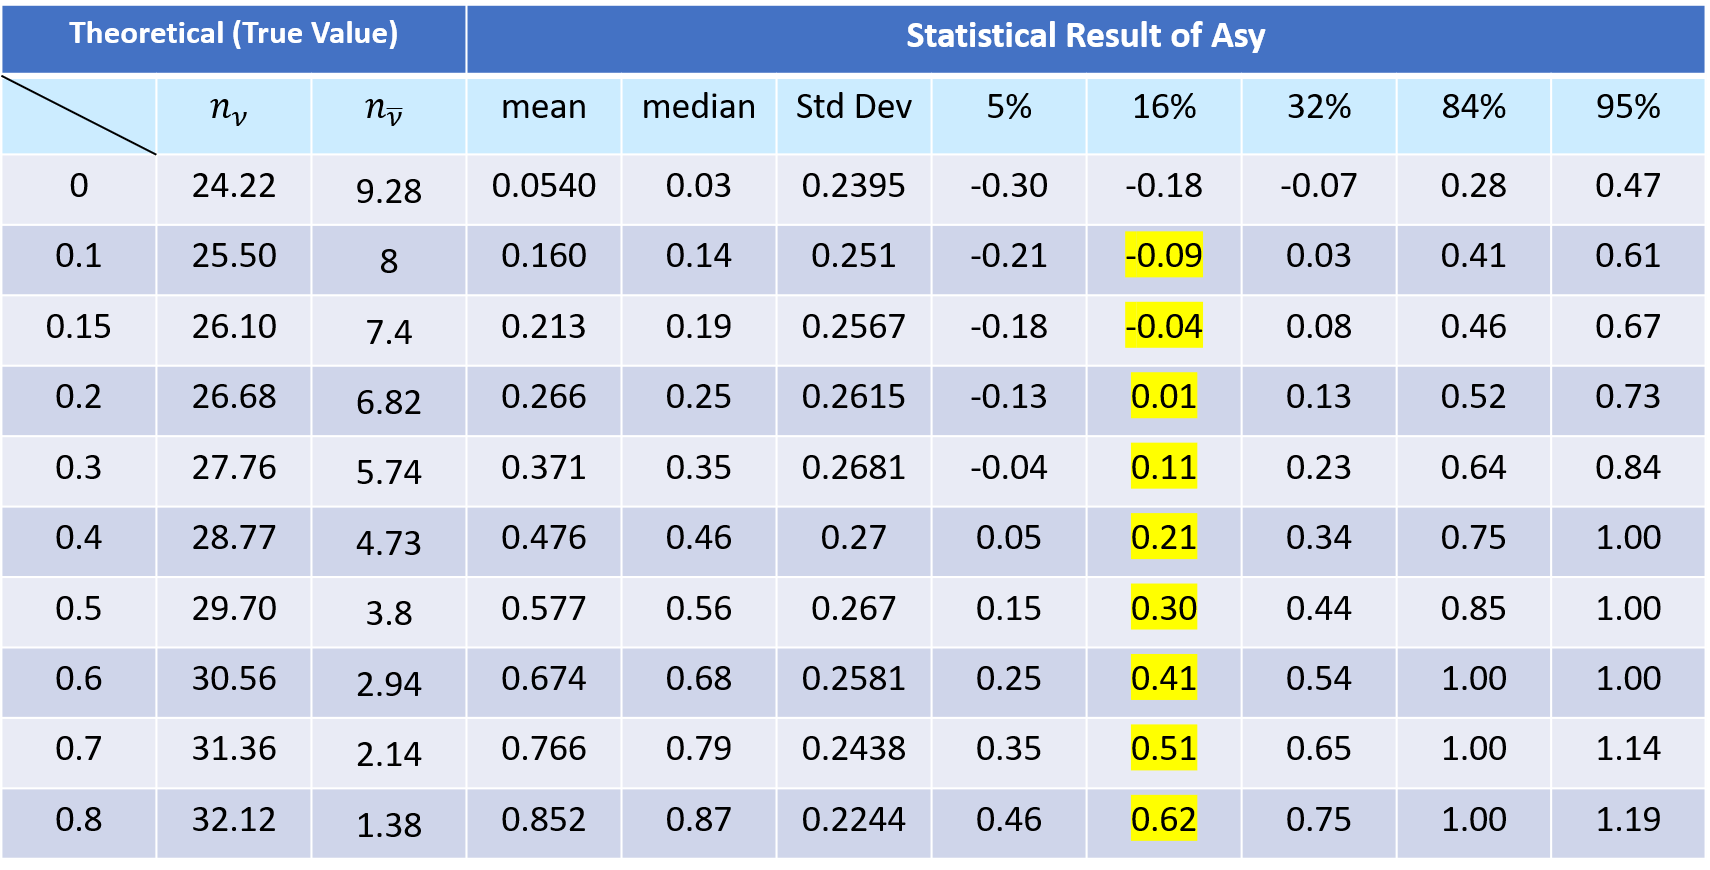
\includegraphics[width=5.5in]{Images/table_bkg_2.png}
\end{minipage}%
\caption{ Statistical result with background}
\label{table_BKG}
\end{figure}



\end{document}

